% Options for packages loaded elsewhere
\PassOptionsToPackage{unicode}{hyperref}
\PassOptionsToPackage{hyphens}{url}
\PassOptionsToPackage{dvipsnames,svgnames,x11names}{xcolor}
%
\documentclass[
  letterpaper,
  DIV=11,
  numbers=noendperiod]{scrreprt}

\usepackage{amsmath,amssymb}
\usepackage{iftex}
\ifPDFTeX
  \usepackage[T1]{fontenc}
  \usepackage[utf8]{inputenc}
  \usepackage{textcomp} % provide euro and other symbols
\else % if luatex or xetex
  \usepackage{unicode-math}
  \defaultfontfeatures{Scale=MatchLowercase}
  \defaultfontfeatures[\rmfamily]{Ligatures=TeX,Scale=1}
\fi
\usepackage{lmodern}
\ifPDFTeX\else  
    % xetex/luatex font selection
\fi
% Use upquote if available, for straight quotes in verbatim environments
\IfFileExists{upquote.sty}{\usepackage{upquote}}{}
\IfFileExists{microtype.sty}{% use microtype if available
  \usepackage[]{microtype}
  \UseMicrotypeSet[protrusion]{basicmath} % disable protrusion for tt fonts
}{}
\makeatletter
\@ifundefined{KOMAClassName}{% if non-KOMA class
  \IfFileExists{parskip.sty}{%
    \usepackage{parskip}
  }{% else
    \setlength{\parindent}{0pt}
    \setlength{\parskip}{6pt plus 2pt minus 1pt}}
}{% if KOMA class
  \KOMAoptions{parskip=half}}
\makeatother
\usepackage{xcolor}
\usepackage{soul}
\setlength{\emergencystretch}{3em} % prevent overfull lines
\setcounter{secnumdepth}{5}
% Make \paragraph and \subparagraph free-standing
\ifx\paragraph\undefined\else
  \let\oldparagraph\paragraph
  \renewcommand{\paragraph}[1]{\oldparagraph{#1}\mbox{}}
\fi
\ifx\subparagraph\undefined\else
  \let\oldsubparagraph\subparagraph
  \renewcommand{\subparagraph}[1]{\oldsubparagraph{#1}\mbox{}}
\fi


\providecommand{\tightlist}{%
  \setlength{\itemsep}{0pt}\setlength{\parskip}{0pt}}\usepackage{longtable,booktabs,array}
\usepackage{calc} % for calculating minipage widths
% Correct order of tables after \paragraph or \subparagraph
\usepackage{etoolbox}
\makeatletter
\patchcmd\longtable{\par}{\if@noskipsec\mbox{}\fi\par}{}{}
\makeatother
% Allow footnotes in longtable head/foot
\IfFileExists{footnotehyper.sty}{\usepackage{footnotehyper}}{\usepackage{footnote}}
\makesavenoteenv{longtable}
\usepackage{graphicx}
\makeatletter
\def\maxwidth{\ifdim\Gin@nat@width>\linewidth\linewidth\else\Gin@nat@width\fi}
\def\maxheight{\ifdim\Gin@nat@height>\textheight\textheight\else\Gin@nat@height\fi}
\makeatother
% Scale images if necessary, so that they will not overflow the page
% margins by default, and it is still possible to overwrite the defaults
% using explicit options in \includegraphics[width, height, ...]{}
\setkeys{Gin}{width=\maxwidth,height=\maxheight,keepaspectratio}
% Set default figure placement to htbp
\makeatletter
\def\fps@figure{htbp}
\makeatother
\newlength{\cslhangindent}
\setlength{\cslhangindent}{1.5em}
\newlength{\csllabelwidth}
\setlength{\csllabelwidth}{3em}
\newlength{\cslentryspacingunit} % times entry-spacing
\setlength{\cslentryspacingunit}{\parskip}
\newenvironment{CSLReferences}[2] % #1 hanging-ident, #2 entry spacing
 {% don't indent paragraphs
  \setlength{\parindent}{0pt}
  % turn on hanging indent if param 1 is 1
  \ifodd #1
  \let\oldpar\par
  \def\par{\hangindent=\cslhangindent\oldpar}
  \fi
  % set entry spacing
  \setlength{\parskip}{#2\cslentryspacingunit}
 }%
 {}
\usepackage{calc}
\newcommand{\CSLBlock}[1]{#1\hfill\break}
\newcommand{\CSLLeftMargin}[1]{\parbox[t]{\csllabelwidth}{#1}}
\newcommand{\CSLRightInline}[1]{\parbox[t]{\linewidth - \csllabelwidth}{#1}\break}
\newcommand{\CSLIndent}[1]{\hspace{\cslhangindent}#1}

\KOMAoption{captions}{tableheading}
\makeatletter
\makeatother
\makeatletter
\@ifpackageloaded{bookmark}{}{\usepackage{bookmark}}
\makeatother
\makeatletter
\@ifpackageloaded{caption}{}{\usepackage{caption}}
\AtBeginDocument{%
\ifdefined\contentsname
  \renewcommand*\contentsname{Table of contents}
\else
  \newcommand\contentsname{Table of contents}
\fi
\ifdefined\listfigurename
  \renewcommand*\listfigurename{List of Figures}
\else
  \newcommand\listfigurename{List of Figures}
\fi
\ifdefined\listtablename
  \renewcommand*\listtablename{List of Tables}
\else
  \newcommand\listtablename{List of Tables}
\fi
\ifdefined\figurename
  \renewcommand*\figurename{Figure}
\else
  \newcommand\figurename{Figure}
\fi
\ifdefined\tablename
  \renewcommand*\tablename{Table}
\else
  \newcommand\tablename{Table}
\fi
}
\@ifpackageloaded{float}{}{\usepackage{float}}
\floatstyle{ruled}
\@ifundefined{c@chapter}{\newfloat{codelisting}{h}{lop}}{\newfloat{codelisting}{h}{lop}[chapter]}
\floatname{codelisting}{Listing}
\newcommand*\listoflistings{\listof{codelisting}{List of Listings}}
\makeatother
\makeatletter
\@ifpackageloaded{caption}{}{\usepackage{caption}}
\@ifpackageloaded{subcaption}{}{\usepackage{subcaption}}
\makeatother
\makeatletter
\@ifpackageloaded{tcolorbox}{}{\usepackage[skins,breakable]{tcolorbox}}
\makeatother
\makeatletter
\@ifundefined{shadecolor}{\definecolor{shadecolor}{rgb}{.97, .97, .97}}
\makeatother
\makeatletter
\makeatother
\makeatletter
\makeatother
\ifLuaTeX
  \usepackage{selnolig}  % disable illegal ligatures
\fi
\IfFileExists{bookmark.sty}{\usepackage{bookmark}}{\usepackage{hyperref}}
\IfFileExists{xurl.sty}{\usepackage{xurl}}{} % add URL line breaks if available
\urlstyle{same} % disable monospaced font for URLs
\hypersetup{
  pdftitle={Github Basics},
  pdfauthor={Greg Chambers},
  colorlinks=true,
  linkcolor={blue},
  filecolor={Maroon},
  citecolor={Blue},
  urlcolor={Blue},
  pdfcreator={LaTeX via pandoc}}

\title{Github Basics}
\author{Greg Chambers}
\date{2025-06-30}

\begin{document}
\maketitle
\ifdefined\Shaded\renewenvironment{Shaded}{\begin{tcolorbox}[sharp corners, interior hidden, breakable, borderline west={3pt}{0pt}{shadecolor}, enhanced, boxrule=0pt, frame hidden]}{\end{tcolorbox}}\fi

\renewcommand*\contentsname{Table of contents}
{
\hypersetup{linkcolor=}
\setcounter{tocdepth}{2}
\tableofcontents
}
\bookmarksetup{startatroot}

\hypertarget{github-overview}{%
\chapter*{Github Overview}\label{github-overview}}
\addcontentsline{toc}{chapter}{Github Overview}

\markboth{Github Overview}{Github Overview}

Github is a widely used tool for managing work and development on
code-based projects. It has several key features:

\begin{enumerate}
\def\labelenumi{\arabic{enumi}.}
\item
  Version control - Github is based on \textbf{git}, a version control
  software. Git allows you to track changes in a project over time, and
  revert to previous versions if problems arise. You can also create
  \textbf{branches} of a project to work on new/experimental features
  without breaking the \textbf{main} code which might need to remain
  functional with no downtime. After completing the branch, the changes
  can be merged into the main code.
\item
  Versatile - You can use Github to collaborate and track changes for
  any text- or script-based project. It is mostly used for hosting codes
  for web/software development or data analysis (SQL, SAS, R, Python),
  but you can also use it for complex
  \href{https://github.com/hendricius/the-sourdough-framework}{documentation
  on sourdough bread making},
  \href{https://github.com/sfu-db/covid19-datasets/tree/master}{data
  storage for public use}, or
  \href{https://github.com/jacobdjwilson/awesome-annual-security-reports}{reports
  on cyber-security threats}.
\item
  Web hosted - Github is a web application that can host public and
  private \textbf{repositories} (or \textbf{repos}). Anyone can see and
  download information on a public repo. Private repos can only be seen
  by individuals with approved access. For our purposes, \ul{no
  sensitive code, PHI, passwords, tokens, or credentials can be stored
  in any repository, even if it is private.} Github is great for working
  on projects for your own use, but it is also a fantastic way to share
  code with other users inside and outside TDH who might find it useful.
\item
  Free - Anyone can create a free Github account. To interact with TDH
  repos, you should create your own account using your tn.gov email and
  two-factor authentication. We can then add you to any TDH CEDEP teams
  in Github, so you can start contributing.
\end{enumerate}

\hypertarget{organization}{%
\section*{Organization}\label{organization}}
\addcontentsline{toc}{section}{Organization}

\markright{Organization}

Our use of Github was only recently approved, so we are still working on
the best way to integrate it into our teams. We have one main
organization, TDH-CEDEP, with several program area subgroups (e.g., SSI,
VH). Once you have your account, an admin can add you to the correct
group(s). You will be able to view/download any public repository, but
you can only see the private repositories for the teams you are a part
of. You can also only make changes to repos for your teams.

If your program area does not have a team in TDH-CEDEP, let us know and
we can create one easily. If you plan on having a lot of users and
repos, it would be good to designate someone on your team to be an
admin, so they can manage access permissions.

\hypertarget{security}{%
\section*{Security}\label{security}}
\addcontentsline{toc}{section}{Security}

\markright{Security}

The following steps should be closely followed in order to adhere to our
agreed upon security protocol with STS:

\begin{enumerate}
\def\labelenumi{\arabic{enumi}.}
\item
  Use your tn.gov email with two-factor authentication when setting up
  your Github account.
\item
  Admins must promptly remove access permissions from users who leave
  CEDEP or transition between teams. They should also perform regular
  user audits.
\item
  Only use Github for projects that need it. You can use Git locally, if
  you just need version control.
\item
  Keep repositories private unless the project needs to be viewable by
  other jurisdictions and/or the public.
\item
  Teams should develop and follow protocols to ensure that no sensitive
  data is published to any repos, public or private. See the security
  page for more details.
\end{enumerate}

\bookmarksetup{startatroot}

\hypertarget{security-details}{%
\chapter{Security Details}\label{security-details}}

STS took a lot of sweet talking before they approved our Github use, so
we want to be on our best behavior (in addition to general data security
concerns). As such, the following practices should be followed when
using Github (expanded from the summary on the first page).

\hypertarget{account-setup}{%
\section{Account Setup}\label{account-setup}}

Use your tn.gov email to create a personal account (can we use our
existing account and add our tn.gov email?). Enable two-factor
authentication for increased security. You will be able to contribute to
your own teams repos using your own account. \ul{{[}section on hosting
your own repos on your own account{]}}

\hypertarget{team-access}{%
\section{Team Access}\label{team-access}}

Admins for the TDH-CEDEP organization must maintain user access to the
correct teams. This includes adding new members to the correct team,
removing team members when they leave their positions, and performing
regular user audits.

\hypertarget{do-you-even-need-github}{%
\section{Do you even need Github?}\label{do-you-even-need-github}}

If you just want version control on a project, you can just use Git
locally. Github is great for sharing projects and working with outside
parties, but if the process is internal, there might not be a point to
hosting it on Github at all.

\hypertarget{public-vs-private-repositories}{%
\section{Public vs Private
Repositories}\label{public-vs-private-repositories}}

The default choice for repositories should be to make them private. More
public repos are just more ways for things to accidentally get published
to the public. That being said, there are reasons why you might want a
repo to be public. Public repos are great for sharing data and code with
other parties, and even having them suggest improvements. You can even
publish data packages that are useful for TDH employees who might not
have their own Github accounts.

It is important to note, that a repository being private should not
affect the sort of information published there. PHI, passwords, etc. are
not allowed in any repo, public or private. {[}should there be a middle
tier of data that can be in private repos, but not public ones ,
e.g.~network paths?{]}

\hypertarget{sensitive-data}{%
\section{Sensitive Data}\label{sensitive-data}}

The following data are not allowed to be published to any Github
repository:

\begin{itemize}
\item
  PHI
\item
  Non-public data (preliminary, data needing suppression, etc.)
\item
  Usernames/Passwords/Credentials
\item
  API tokens
\end{itemize}

In order to prevent this data from getting into Github, remove it from
your codes and become used to excluding it from your work without
consideration for if it will end up in Github. It is especially easy to
leave notes or comments in code about test cases or outliers that might
need to be deleted before saving a file.

You can also use gitignore functionality to hide certain files from Git,
which can help when you need data for a code to run on your machine, but
you don't want it in the version history that goes in Github.

{[}Consider a middle tier of info that can be in private but not public
repos{]}

\hypertarget{removing-sensitive-data-from-a-repo}{%
\subsection{Removing Sensitive Data from a
Repo}\label{removing-sensitive-data-from-a-repo}}

If sensitive data gets pushed to Github, we need to take it down as fast
as possible. Follow the following steps:

\begin{enumerate}
\def\labelenumi{\arabic{enumi}.}
\item
  Notify an admin
\item
  Make the repository private (if it isn't already)
\item
  Edit the repo to remove the sensitive data
\item
  Edit the version history to remove the sensitive data {[}develop
  guidance because this can be complex{]}. Note information needed for
  follow-up investigation (time published and removed, author, file
  source, etc.)
\item
  Notify anyone else who needs to know (e.g., HIPAA protocol)
\item
  Determine steps to make the repo public again (if appropriate)
\end{enumerate}

\bookmarksetup{startatroot}

\hypertarget{github-basics}{%
\chapter{Github Basics}\label{github-basics}}

This section covers the basics of how Github works. There are a lot of
resources online that can also help you understand. Github is a website
that is based on Git. Git is a common version control software.

\hypertarget{what-is-git}{%
\section{What is Git}\label{what-is-git}}

Git was developed to track changes in software over time, with multiple
people working on the same code at once. You can download Git onto your
PC and use it without worrying about Github at all. The diagram below
shows how a project is developed using Git version control.

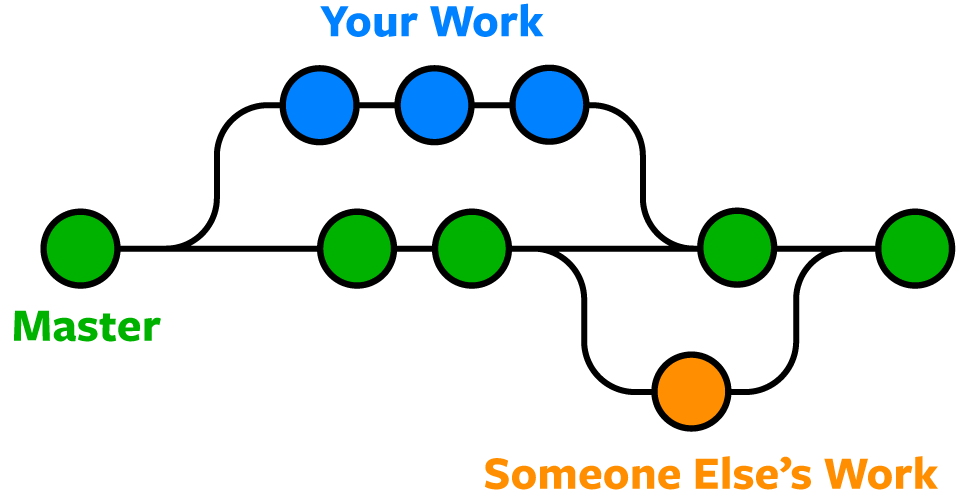
\includegraphics{index_files/mediabag/git-branches-merge.png}

The project starts in an initial state, called the main (sometimes
master) branch. In the diagram above, the main branch is colored green.
Each circle is the code at a point in time, referred to as a commit.
When a change is made to the code, you must choose to commit the change
to the version history. You will also be asked to write a short
description of what you changed or added. Uncommitted changes are
considered staged, since they are waiting to be accepted or rejected.

For minor fixes, like correcting a typo, you could edit the main branch
of code and commit the changes to it directly. But sometimes a change is
more involved, and working on it will take time. Furthermore, sometimes
you need to make changes to the foundations of a script that render it
non-functional, but other people rely on the code to keep running. In
this case, Git allows you to create a branch (in blue and orange above).
Branches are a copy of the code that is separate from the main,
functional code. You can then make edits to your branch without breaking
the functional code. When you have finished work on the branch, you can
then merge your changes into the main branch. In the diagram above, the
blue branch took three commits to finish, whereas the orange commit only
took one.

When making a commit, or merging a branch into main, you will have the
opportunity to review the old version of the code and the new version.
This is so each change is highlighted and looked over before it is added
to the version history. The above process allows for complex projects
with several contributors to be developed with a clear history of who
did what and when, with the ability to go back to previous versions of
the project, if need be.

A Git project can consist of one or more files that are located together
in a folder. This location, and the files in it are known as a
repository, or repo. All the files and subfolders in the repo are
included in the project's version control. Git can be used by typing
commands into a terminal or command prompt, but other tools (Github,
Rstudio, etc.) provide a user interface that can make getting started
easier.

Here are the key terms from the description above:

\begin{itemize}
\item
  Version control - Tracking, recording, and organizing changes to a
  project over time
\item
  Git - a version control software
\item
  Main - The base version of a project
\item
  Branch - a copy of the main project, where changes can be made
\item
  Staged Change - an edit to a file in a repo that has not been
  committed
\item
  Commit - Officially adding a change to the version history (to the
  main project, or to a branch)
\item
  Merge - Adding changes from a branch back into the main project
\item
  Repository - A location that contains the files and folders that make
  up a project
\end{itemize}

\hypertarget{what-is-github}{%
\section{What is Github}\label{what-is-github}}

As stated above, you can use Git locally on your own computer. In this
case, you are working on a local repository, or a project on your own
computer. Github is a remote repository; a place to store the code that
is not your own computer. This allows the code, with all its version
history, to be available to everyone (a public repo), or github users
with certain permissions (a private repo).

You can take an existing local Git repository and push it up to Github.
Most code editors can easily integrate with Git and Github, to
facilitate communication between your local repo and Github's remote
repo. After working on some changes to the code and making one or more
commits, you can push the changes up to Github (syncing the Github repo
to align with your local repo). Conversely, you can pull the current
version of the project from the Github repo to your own local repo in
order to make changes off of it. This is useful for projects with
multiple collaborators. You will typically all use Github as the hub for
development; pull down the current version of the project with the most
recent changes from others, make and commit your changes locally, then
push them back to Github. Then others can do the same.

\includegraphics{local_remote_repo.webp}

Pulls and pushes happen to branches of a repository, but you should
start off by working on a small project with only a main branch. Here is
an example of the code review panel in R for a small documentation
change:

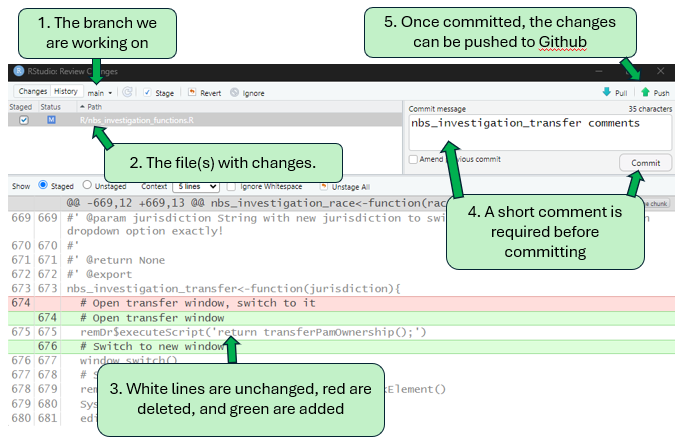
\includegraphics{images/commit_review_R.png}

Here are the key terms from the description above:

\begin{itemize}
\item
  Local Repo - A group of files and folders that make up a project,
  stored on your own computer
\item
  Remote Repo - A repo stored on a remote server, like Github
\item
  Pull - Copying a remote repo from Github to a local repo on your
  machine
\item
  Push - Updating a remote Github repo to reflect commits made to your
  local repo
\end{itemize}

\hypertarget{common-elements-of-a-repo}{%
\section{Common Elements of a Repo}\label{common-elements-of-a-repo}}

Many different file types can be placed into a repo, but there are some
items which are commonly used to make working with Git/Github easier.
None of these are strictly required (except for a license, potentially),
but you should use them.

\hypertarget{readme}{%
\subsection{Readme}\label{readme}}

A file that explains the purpose of the project, and any useful
documentation on how to use the code inside. In Github, readme files
should be markdown documents (i.e., readme.md). When structured this
way, the readme information will be rendered in the Github repo.

\hypertarget{gitignore}{%
\subsection{.gitignore}\label{gitignore}}

The .gitignore file allows you to specify files and folders that should
not be included in the version control tracking. These files can be
housed inside the repo folder, and could be critical to the functioning
of the code (e.g., important data for analysis), but changes to these
files are not tracked, and they won't be pushed to Github. Specific
files can be listed in the .gitignore, or patterns that exclude multiple
items (e.g., all PDFs, all files with ``PHI'' in the name, all files in
a subfolder)

\hypertarget{subfolders}{%
\subsection{Subfolders}\label{subfolders}}

The main folder of a repo can store files, but it can also help to
organize files into subfolders. Common subfolders are for data, scripts,
or images

\hypertarget{license}{%
\subsection{License}\label{license}}

Since the code put into public repositories can be seen and copied by
anyone, you likely need a license that describes how the code can be
used by others {[}what is the TDH default license? Does this need to be
mentioned in security?{]}.

\hypertarget{credentials}{%
\section{Credentials}\label{credentials}}

You will need to link your computer to your Github account. Options
include:

\begin{itemize}
\item
  Git terminal
\item
  Git UI {[}maybe?{]}
\item
  IDE capabilities

  \begin{itemize}
  \item
    RStudio -
    \url{https://usethis.r-lib.org/articles/git-credentials.html}
  \item
    SAS -
    \url{https://communities.sas.com/t5/SAS-Communities-Library/How-to-connect-SAS-to-your-Git-profile/ta-p/772570}
  \item
    VSCode
  \end{itemize}
\end{itemize}

You should only need to set your credentials once {[}pending security
concerns{]}. Once set, any commits/pushes/pulls/etc. will include your
name, and you will have the ability to access private repositories for
your teams.

\bookmarksetup{startatroot}

\hypertarget{extra-resources}{%
\chapter{Extra Resources}\label{extra-resources}}

\hypertarget{other-github-summaries}{%
\section{Other Github Summaries}\label{other-github-summaries}}

\begin{itemize}
\item
  \url{https://www.coursera.org/articles/what-is-git}
\item
  \url{https://digital.gov/resources/an-introduction-github}
\end{itemize}

\hypertarget{rstudio-integration}{%
\section{RStudio Integration}\label{rstudio-integration}}

\begin{itemize}
\item
  \url{https://happygitwithr.com/rstudio-git-github.html}
\item
  \url{https://rfortherestofus.com/2021/02/how-to-use-git-github-with-r}
\item
  \url{https://www.epirhandbook.com/en/new_pages/collaboration.html}
\end{itemize}

\hypertarget{sas-integration}{%
\section{SAS Integration}\label{sas-integration}}

\begin{itemize}
\tightlist
\item
  \url{https://documentation.sas.com/doc/en/egug/8.3/p078cl08fol7hkn11a8nf1f9izq7.htm}
\end{itemize}

\bookmarksetup{startatroot}

\hypertarget{references}{%
\chapter*{References}\label{references}}
\addcontentsline{toc}{chapter}{References}

\markboth{References}{References}

\hypertarget{refs}{}
\begin{CSLReferences}{0}{0}
\end{CSLReferences}



\end{document}
